\documentclass[border=4pt]{standalone}
\usepackage{pgfplots}
\pgfplotsset{compat=1.18}

\begin{document}
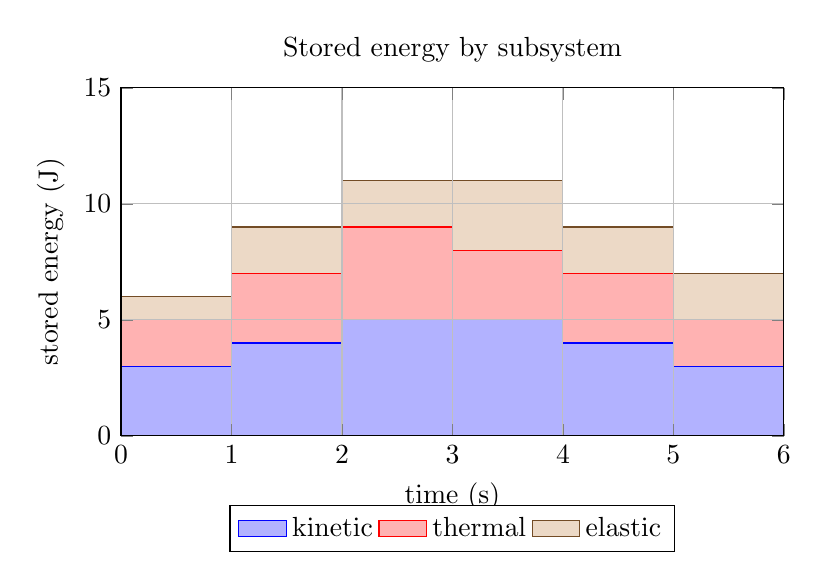
\begin{tikzpicture}
  \begin{axis}[
    const plot,
    stack plots=y,
    area style,
    width=10cm,
    height=6cm,
    xmin=0,
    xmax=6,
    ymin=0,
    ymax=15,
    enlargelimits=false,
    xtick={0,1,2,3,4,5,6},
    xlabel={time (s)},
    ylabel={stored energy (J)},
    title={Stored energy by subsystem},
    grid=major,
    legend style={at={(0.5,-0.2)},anchor=north,legend columns=-1}
  ]
    \addplot coordinates {(0,3) (1,4) (2,5) (3,5) (4,4) (5,3) (6,2)} \closedcycle;
    \addplot coordinates {(0,2) (1,3) (2,4) (3,3) (4,3) (5,2) (6,2)} \closedcycle;
    \addplot coordinates {(0,1) (1,2) (2,2) (3,3) (4,2) (5,2) (6,1)} \closedcycle;
    \legend{kinetic,thermal,elastic}
  \end{axis}
\end{tikzpicture}
\end{document}
